\chapter{Design}

Once the requirements have been decided, is time to make the design of the system
that will do all needed to cover them. First, we are going to take a look over
the general architecture, the distribution of the domain of the services and
how to delimit their behavior and communications with each other, by after,
take a look to each one to know how to work in each domain and how have been solved all problems
that this design present.

\section{Responsabilites distribution}

At the moment that we decided split the functionality of the system between
services we found the problem that how to decide which is the domain
\intro
At the moment that we decided split the functionality of the system between
services, we found the problem that how to choose which is the domain of each one.
In the majority of the cases, we are beginning from a monolithic system that we
want split, in this instance, is some like this but at first, it was thought to be splited.
\intro
In a common app (whatever kind of it) we have three well-defined layers, user
interface, logic and storage, something as common MVC\footnote{Model–view–controller
(MVC) is a software architectural pattern for implementing user interfaces on
computers. It divides a given application into three interconnected parts in
order to separate internal representations of information from the ways that
information is presented to and accepted from the user, user interfaces pattern,
introduced by Trygve Reenskaug into Smalltalk-76 at Palo Alto Research Center in the 1970s}
A part of user interface make the necessary to present the info and offer the
way to interact with this to the user while the logic layer do this possible
doing the logic steps to work with data structures saved in some kind of storage.
\intro
There are some frameworks as Django wherein all this layer can be developed
together, is not strange their popularity, but if we use other as AngularJS
this only help us in the user interface layer, not in the rest, but for other
hands have another advantage.
\intro
So, that as it may, this would be the more simple schema to start to work in
our domain, with the difference that we work with service instead of layers in a
single program, but essentially, the concept is the same.
\intro
As we can see in the next picture, we will have a user interface, when  will
built all views and controllers that work with this to build a complete user
interface, a logic section layer, here labeled as APIGmService (as a first
approach) that will do the logic of the system, transform the data,
restructuring and offering the interaction form UI to database.
And at end, the database system, mainly an engine of the database and the drivers
necessary to work with them.

\begin{figure}[H]
  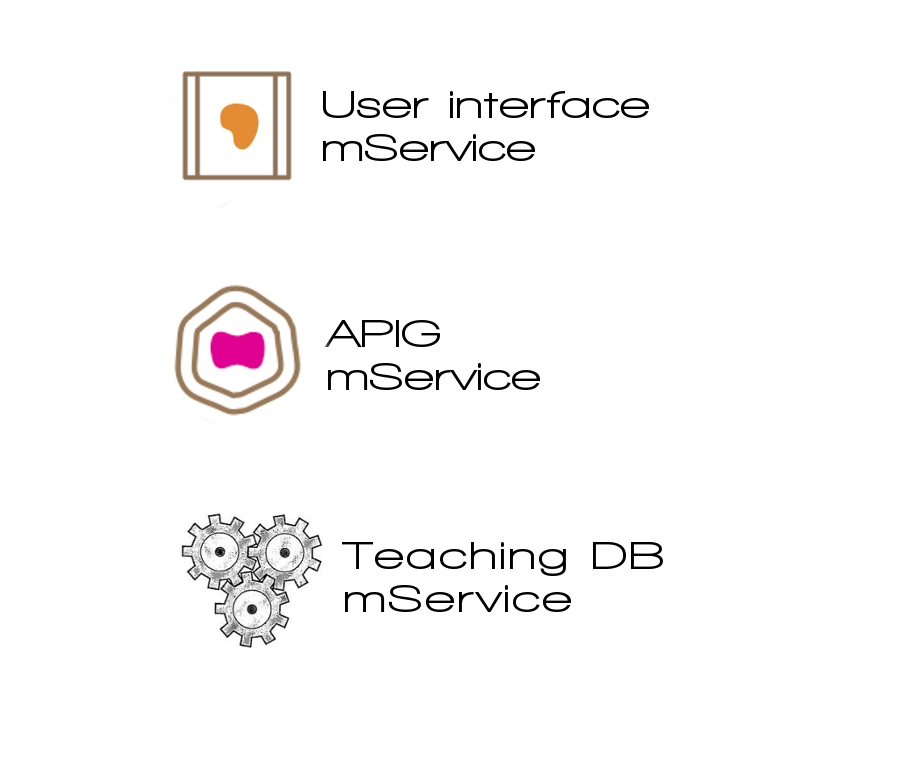
\includegraphics[scale=0.25]{img/graphics/initial_microservices_distribution.png}
  \centering
  \caption{Basic layers in common app.}
\end{figure}

\noindent As we can imagine this work fine, is compact and stable when we are talking about
the same code on the same machine but now we are going to split that in
different services, maybe running at different places and maybe in different
languages, so when we talk about divide the domain is about split the logic with
the database access layer.
\intro
Next picture shows us perfectly what are talking about. This is an example
of migration from monolithic to microservices from Nginx resources.

\begin{figure}[H]
  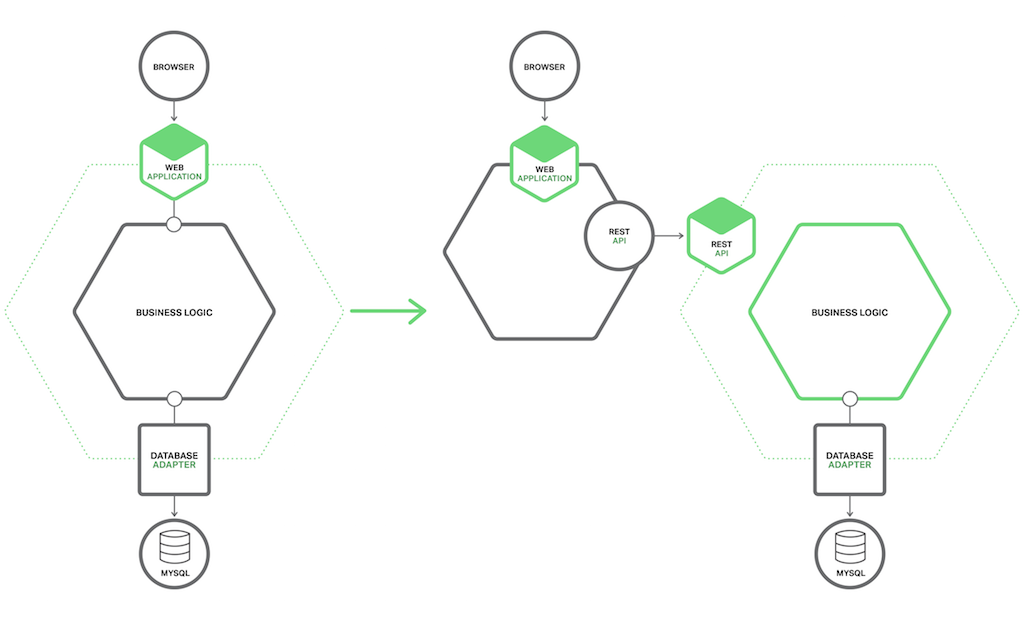
\includegraphics[scale=0.35]{img/graphics/refactoring.png}
  \centering
  \caption{Monolithic to microservices, from nginx resources. }
\end{figure}

\noindent So, for us, each service will always be mainly the same components,
communication protocol and logic layer while database layer will always be optional,
a service can do some logic without need a database, imagine a simple service
to do several calculations or consume the data from another service or act as
third party services gateway, a social network, a payment service, whatever.
\intro
Coming back again to our problem we have decided to split all the back end in
four services that will cover the domain of the problem, following a Domain
Driven Development principles. Each one will be described with details after,
for now, only some reasons that why is so. We need a logic part that controls
any system call, some as the gateway that acts as a dispatcher of requests, that
call to the service (maybe not only one) that can help it to resolve the requests
and give back the info.
\intro
For another and, we need cover all requirements specified,
and to achieve this we are going to design three services that split all logic
issues, it will be \textbf{Teaching Database microService}, \textbf{Students Control}
and \textbf{Analysis microService}. All toguether compose the backend of the app,
toguether with other service that will enlarge the functionality of our project
in the future.
\intro
So, as a big picture, the backend of our service would look like this, some
services with approximately the same form (in the pictur only three, is the same).

\begin{figure}[H]
  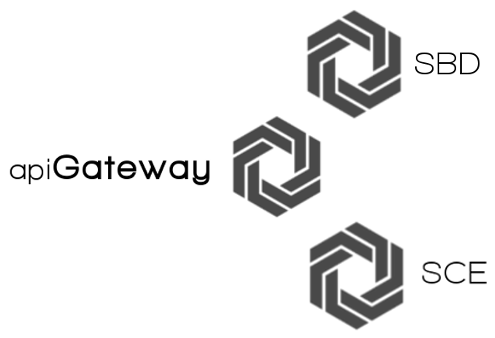
\includegraphics[scale=0.25]{img/graphics/backend.png}
  \centering
  \caption{Some as the first approach of the system.}
\end{figure}

\noindent Once that the architecture is clear and the services are well defined
(not their behavior, only their domain) we must have clear how this services will
be deployed in the platform or infrastructure chosen because the selection can
modify the way to design the services.
\intro
So in our case, of all possibilities that we have already discussed before we
only consider two as acceptable, Google and Amazon infrastructure, so as you
know already, Google was the selected, so we need design our services to run
inside of it and this mean that we need how configure our services.
\intro
As we always evaluate some options, we have done a simple design to see what
will be the infrastructure and design required, first in Amazon Web Services.
\intro
In this case, as the code must run into the container we would need configure
all our services as Docker Containers and to use the service Amazon EC2 Container
Service to deploy them. And our gateway service could be deployed in another
container or could be used a specific service called API Gateway Service with
Lambda Service, both services was launched by Amazon when they saw that this
pattern was really common in all projects, and they design this service to save
efforts to developers (even though it have some drawbacks as for example that you
do not try it in local, at least for now but is sure that will be solved).

\begin{figure}[H]
  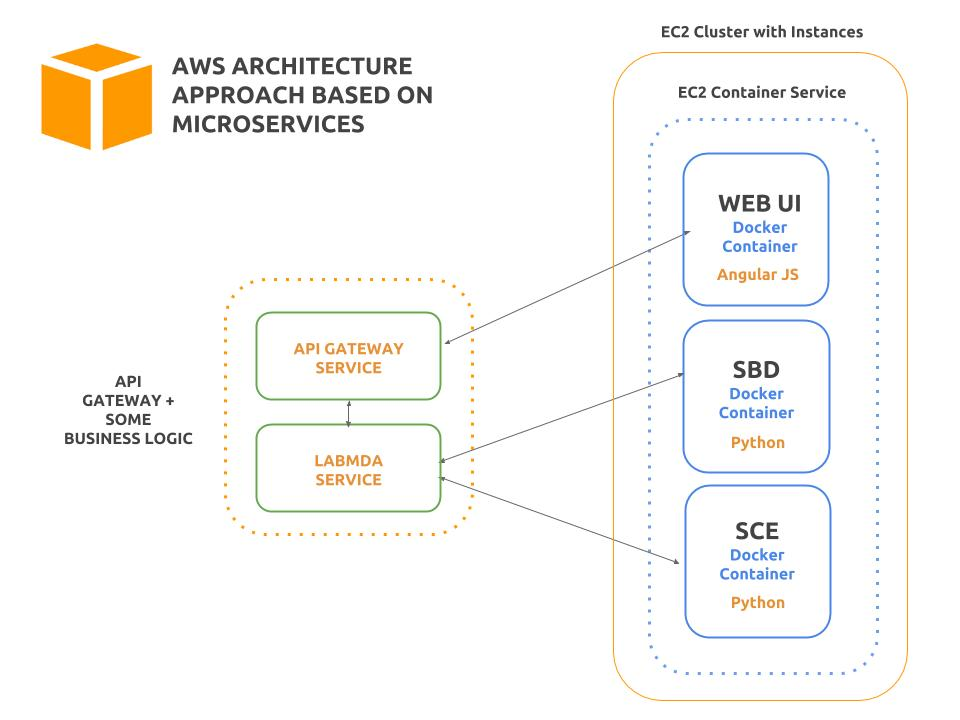
\includegraphics[scale=0.35]{img/graphics/aws_approach.jpg}
  \centering
  \caption{Approach in Amazon Web Service infrastructure.}
\end{figure}

\noindent The goal of this study was compare the facilities or drawbacks of each platform
(doing a little bit deep study that only to take a look over the solutions each
one offered), and the drawbacks of AWS for this kind of "amateur" project was too.
\intro
Come back to GAE, the deploy must be different because there are not docker
container, we only have speciall sandbox to run our code with some special
characteristics (as wee commented before). But, the architecture does not vary
significantly between both architectures, as could not have been otherwise.
If this not so, microservices and their platform independence would not have sense.
\intro
So, focused on GAE, the services must be deployed and developed (nothing else of
some changes in the code) as modules (now called services by GAE) and this can
(and must) put joined in GAE applications. So, as the platform are thought and
to adjust this to our requirements we are going to launch two apps, one only with
the user web interface service (front end) and another with the group of services
that compound the backend, (here GAE app 2).
You can see the distribution in the next picture.

\begin{figure}[H]
  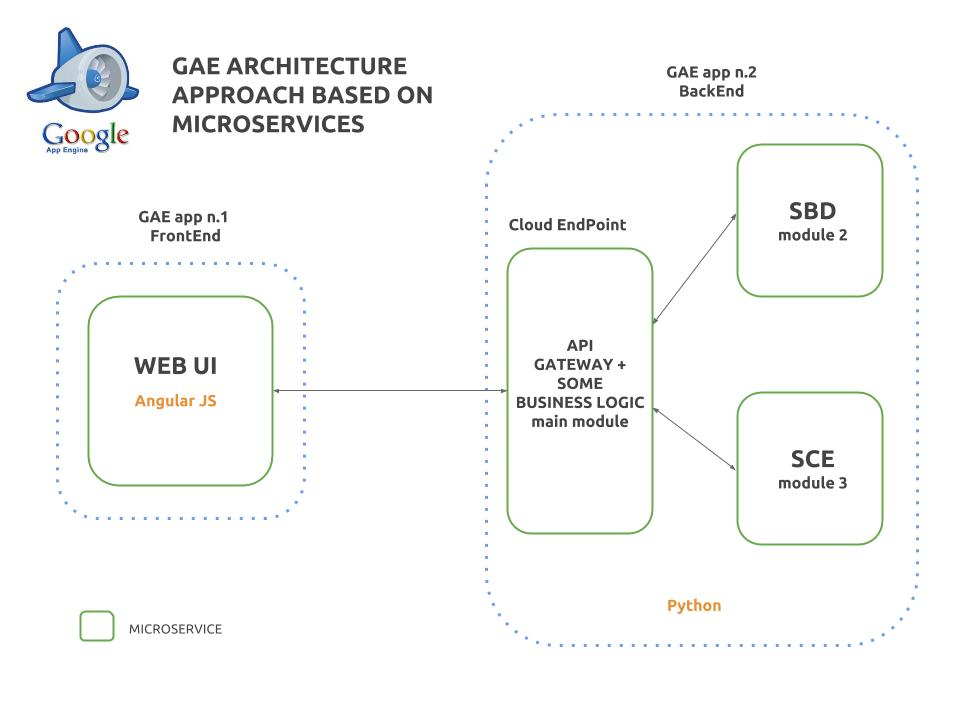
\includegraphics[scale=0.35]{img/graphics/gae_approach.jpg}
  \centering
  \caption{The same approach in Google App Engine infrastructure.}
\end{figure}


\subsection{Be more realistic}

As is esay to imagine, is needed a lot of services to complete all requirements
of the project, and presented here is only the most important because define the
core of app and their structure but of course are necessary a lot more.
Only thinking about security and authentication is easy to see that is necessary
other services to check this, but as is a standard service (not taking part in
the design of the app) not will be developed now and neither explained here.
Their goals are to ensure the authentication of the user and provide the user
authorization of different parts of the app. So, this will be Authorization \&
Authentication microService.
\intro
On another hand, there are two more functionalities must be developed as soon as
possible in the next iterations, a files storage, and a messaging service.
Both are necessary for a more advanced stage of the deploy, not now, but essential
in the final product. The next picture shows you all services, developed in this
phase and the planned.

\begin{figure}[H]
  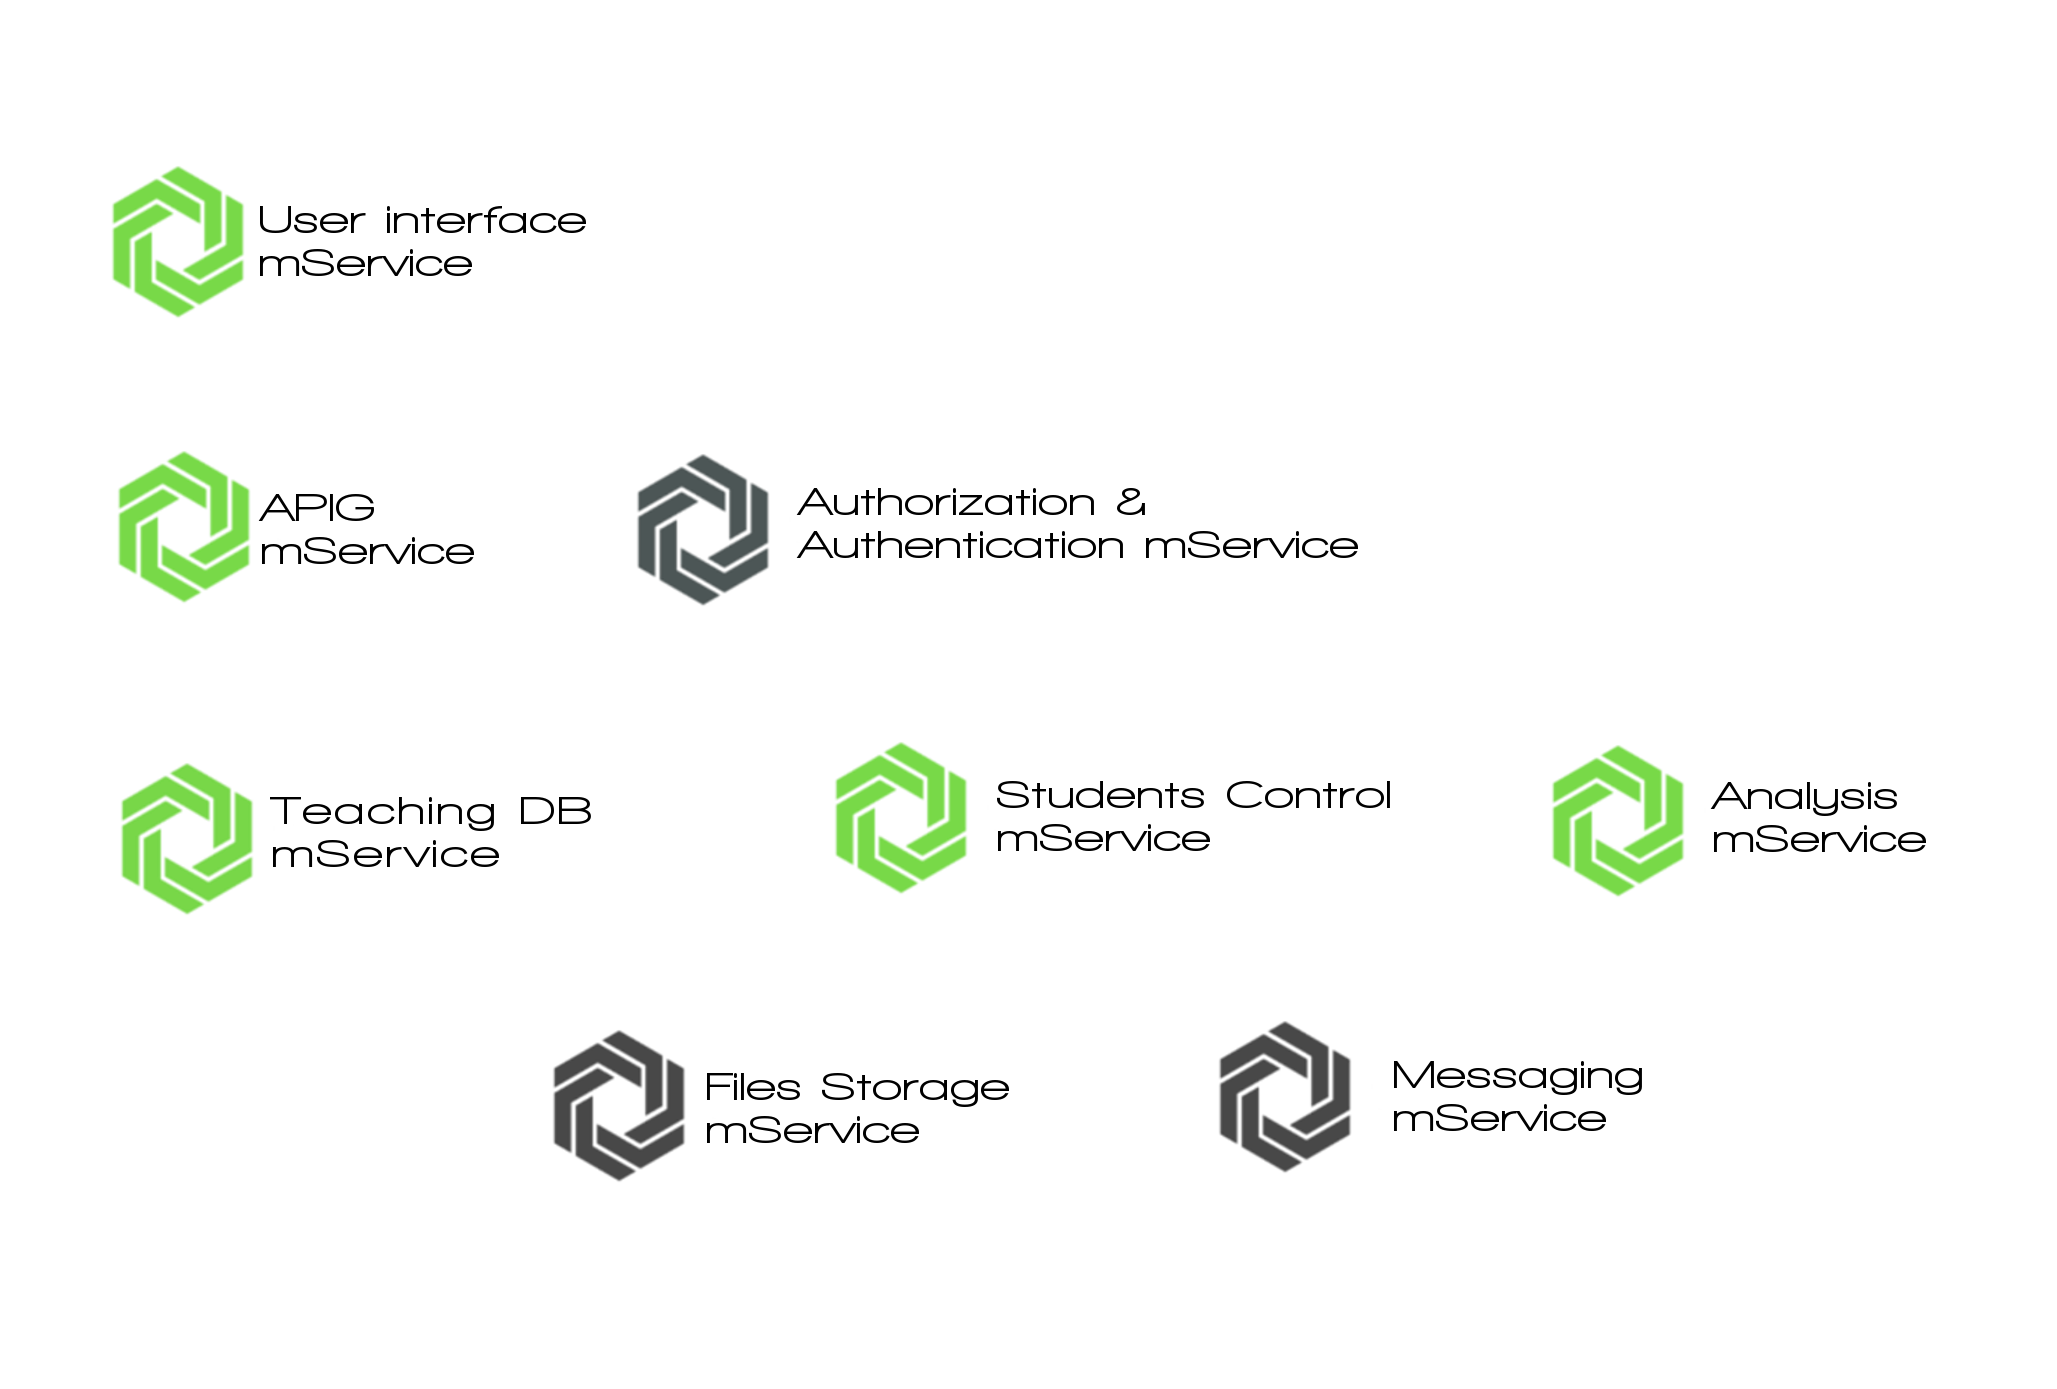
\includegraphics[scale=0.22]{img/graphics/final_microservices_distribution.png}
  \centering
  \caption{Group of microservices of SMS launched and planned.}
\end{figure}

\noindent Next picture shows us a more realistic snap of the deployment, with
the services, technologies, tools and third party services consumed.
We can see how SCmS need G Cloud Datastore, TDBmS Cloud SQL (for example) and
all technologies related.

\begin{figure}[H]
  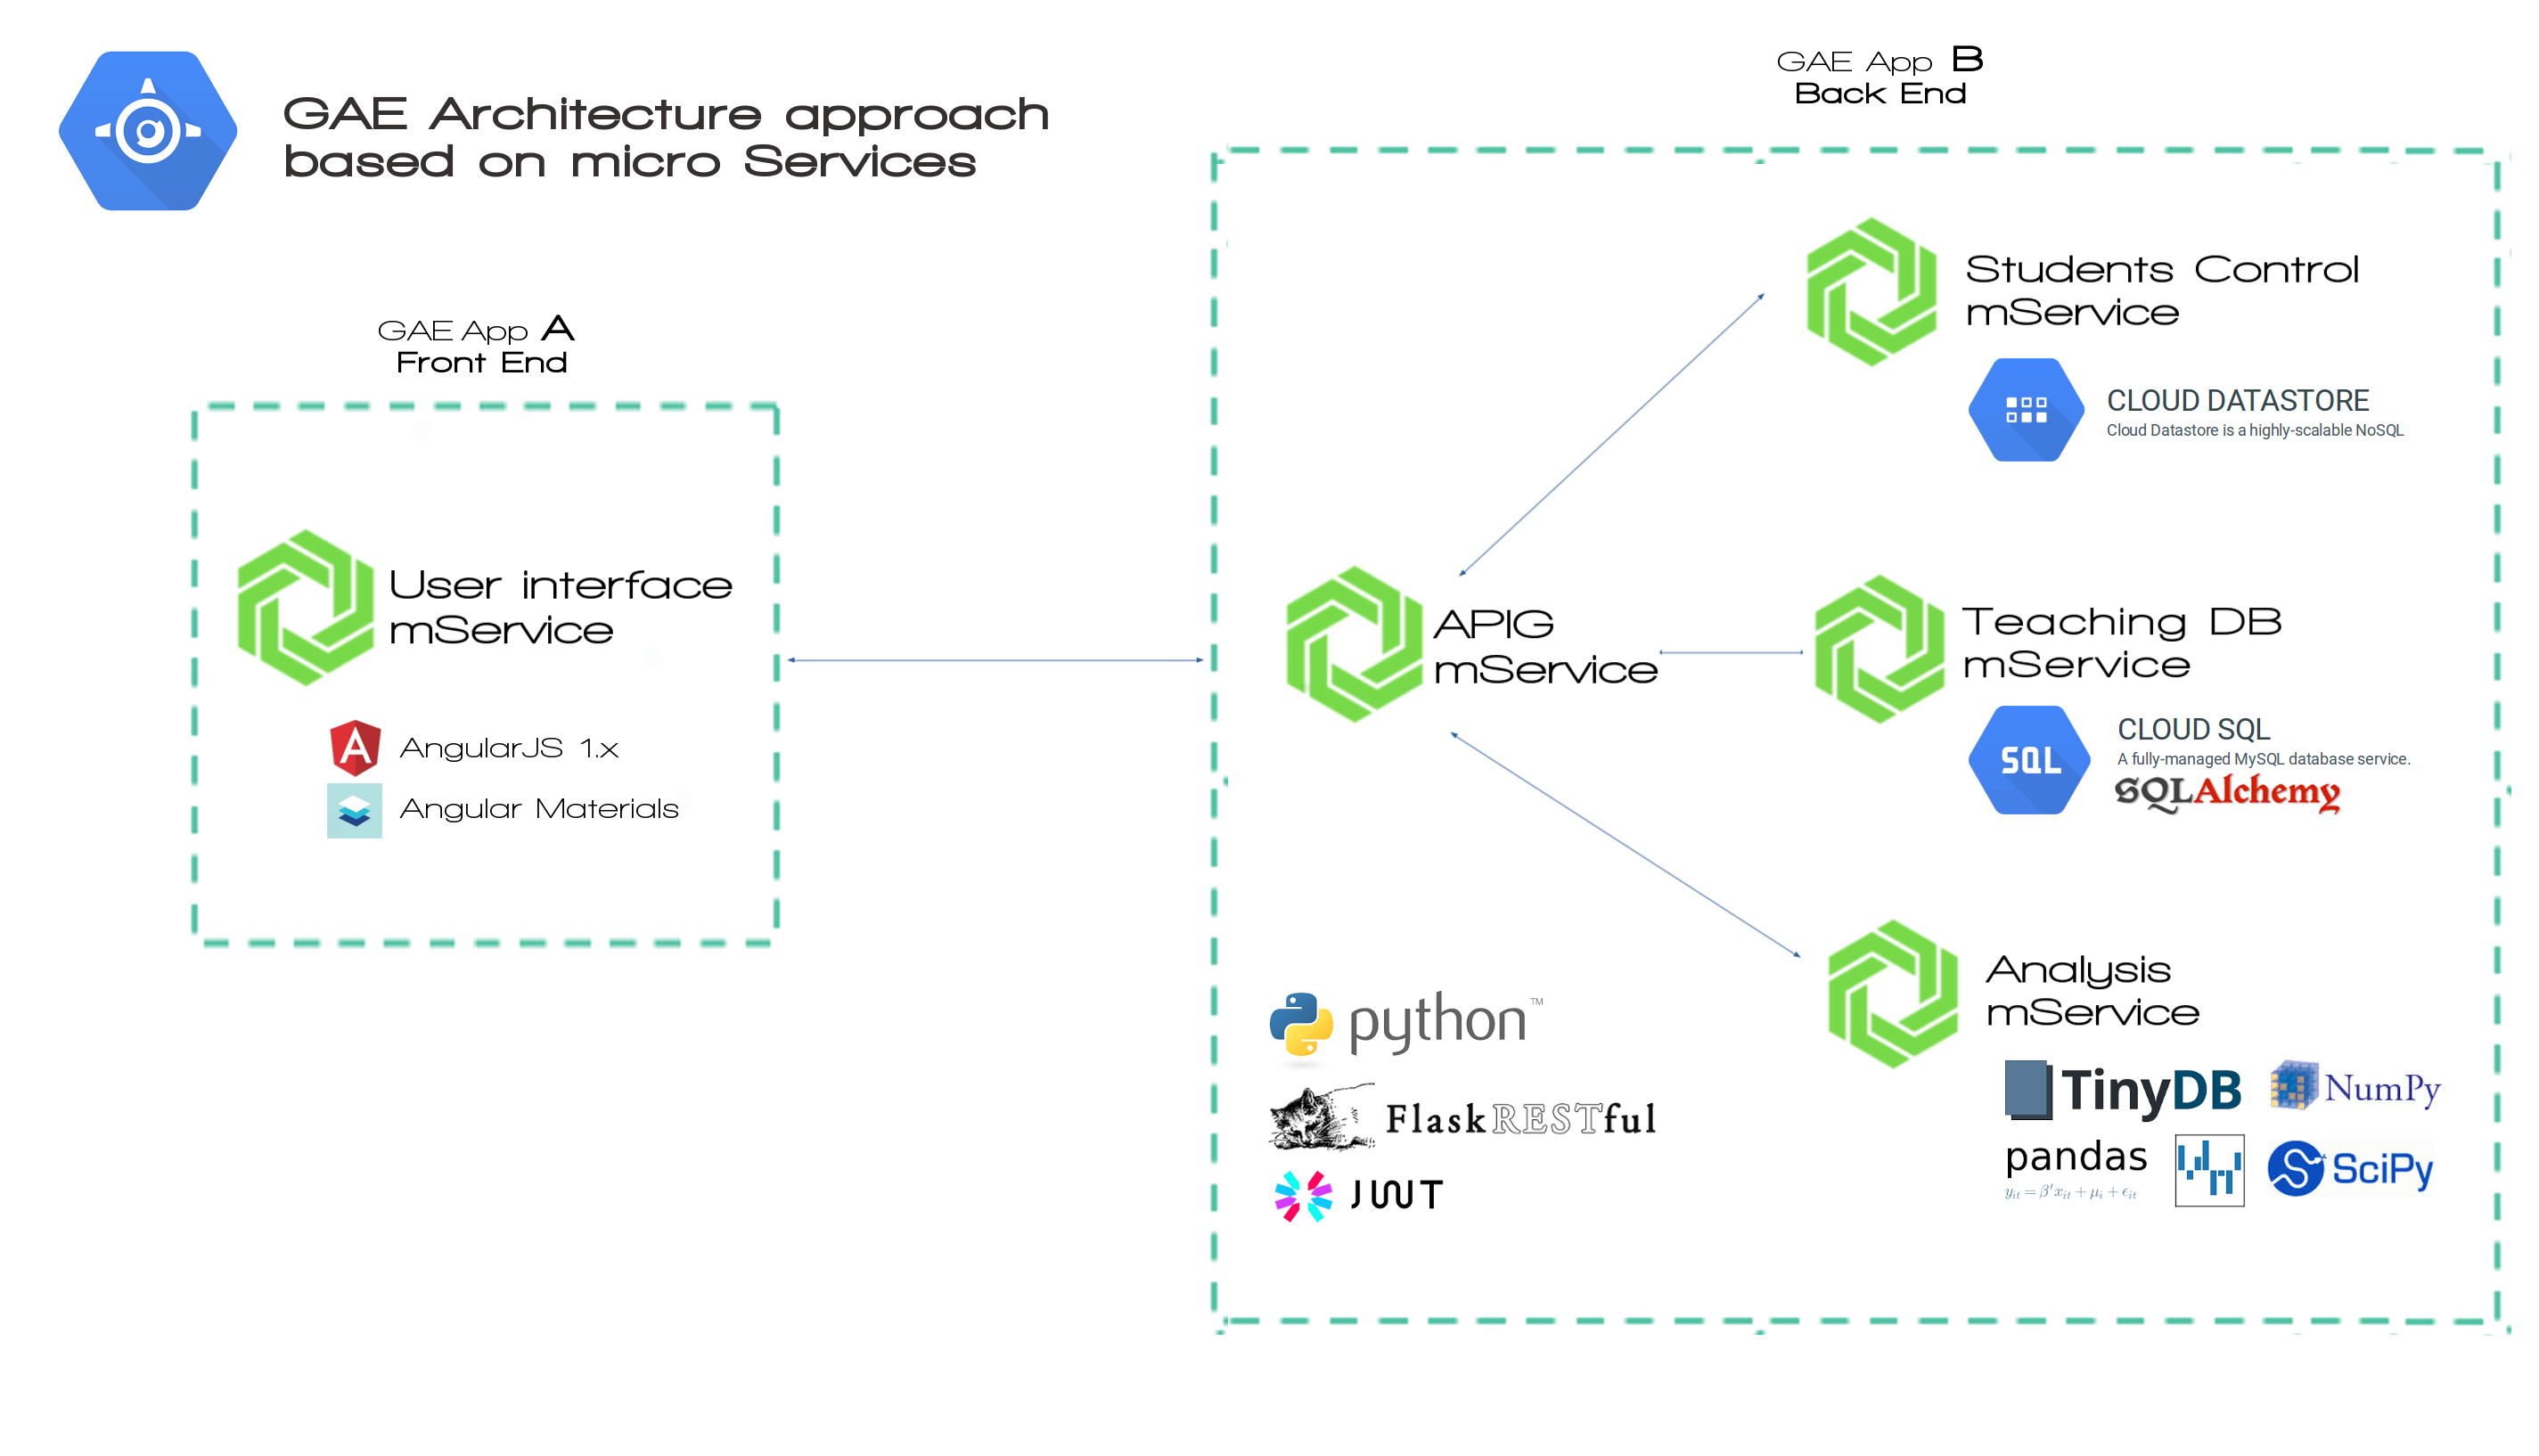
\includegraphics[scale=0.15]{img/graphics/GAE_final_architecture.png}
  \centering
  \caption{Final snap of the distribution of the services with their technologies.}
\end{figure}

\noindent And will be our roadmap to follow, without any service needed to obtain a pre-alfa
product version that satisfy minimum requirements at this point.


\section{API standar status codes}

When we design an API over HTTP we are assuming that we are going to use standard
status code of this protocol (HTTP/1.1 in particular) and is useful that from beginning
all team knows what code will be used and the meaning. The next table shows us which is these,
obviously, there are a lot of more, but this is most important for us.

\begin{table}[H]
\centering

\begin{tabular}{@{}lllllll@{}}

Status Code & Meaning & Use/Behavior\\
\midrule

200 & Ok & Any request that returned content.\\
201 & Created. & Not return content and the item has been saved.\\
204 & Ok without body. & Call with success without content. \\
404 & Not found. & Element not founded.\\
422 & Unprocesable entity. & Bad body at request.\\
500 & Server error. & Any unknown kind of server error.\\

\end{tabular}
\caption{HTTP1.1 Status Code common used}
\label{my-label}
\end{table}

\noindent And as is known, the numbers have a specific meaning and it will
be useful to know just in case another will appear.

\begin{table}[H]
\centering

\begin{tabular}{@{}lllllll@{}}

Class & Meaning\\
\midrule

2xx & Successful\\
3xx & Redirection\\
4xx & Client Error\\
5xx & Server Error\\

\end{tabular}
\caption{HTTP1.1 Status Code first digit meaning}
\label{my-label}
\end{table}


\section{Pesistence Strategy}

When we are talking aobut persitency that meaning how the data that change
their state in the database is manage. Obviously we are talking of the changes
between created, deleted and the between states.
\intro
Is been identified three ways to do this:

\begin{itemize}
  \setlength{\itemsep}{0pt}
\item \textbf{Non persistence}
      \intro
      When a item is updated or deleted any information of the last state remain.
      \intro
\item \textbf{Half persistence}
      \intro
      When a data is logically erased, the data remain in the database but will never
      accesible by the user. In this case is isseful if we want develop some mechanism
      to redo acctions, in this case only deletion actions.
      \intro
\item \textbf{Complete persistence}
      \intro
      When not only the elements erased can be restored, all items can be restored in
      any point of the hisory of the system. This is the more complex mechanism to persistence
      but also the most powerfull and usseful for the users, because as in a simple
      text editor allow do an infinite redo over acctions realized.

\end{itemize}

\noindent Afte study all options have been decided use the second approach, and to achieve
this is necessary get some kind of metadata pluged to our objects stored in databases
to control their state in all moment.
To do this has been designed this metadada pattern for all objects saved in any
service or database:

\begin{lstlisting}[language=python,frame=none]
  Metadata parameters
  createdBy       INT,
  createdAt       DATETIME,
  modifiedBy      INT,
  modifiedAt      DATETIME,
  deletedBy       INT,
  deletedAt       DATETIME,
  deleted         BOOL,

\end{lstlisting}

With it we get a simple way to save logically deleted items, that allow us
develop a simple way to recovery this if user want, and not only this, also
a system to know who do the actions, who save, delete or update an item and
also when, a lot of data very usefull in many ways.


\section{API Gateway microService}

On the other had with docs something similar happens, don't have sense
write a doc defining the behaviour of all sections of api gateway
if this doc already exists in each service. It's redundant and complex
to mantain. Because of this a simple approach is link the docs to
services docs, so the task of write it relegate to them.


\begin{center}
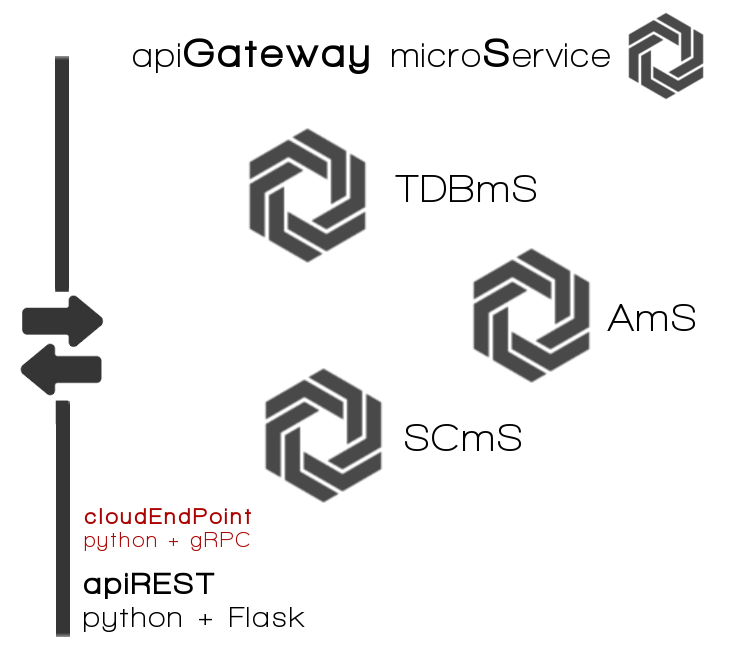
\includegraphics[scale=0.35]{img/graphics/apigateway.png}
\end{center}

\subsubsection {API Definition}






\section{Teaching Data Base microService}

\subsection{Domain and design}

This mService offers the managment of the teaching of the center.
This means that persist in a relational database all relations between
teachers, students, subjects, etc, and all resource availables to
make this posible throuhg an api.\bigskip

This like the rest offers his resource throuhg an api writed in Flask
(follow the same architecture that all).

The engine to save all these relations is MySQL, for many reasons,
mainly because is the best known engine and in which it has some experience
and also because GCP offers as a cloud product Google Cloud SQL Databases.
Until recently only offerts MySQL but now (since March of 2017) they
offer also PostgreSQL.

Access Library design

In the old version it was a little ORM that offers simple methods
to access data transform this in SQL raw sencentes. Now this library
is only a wraper of the SQLAlchemy to keep apart the apirest of the
service to the database access layer.

\begin{center}
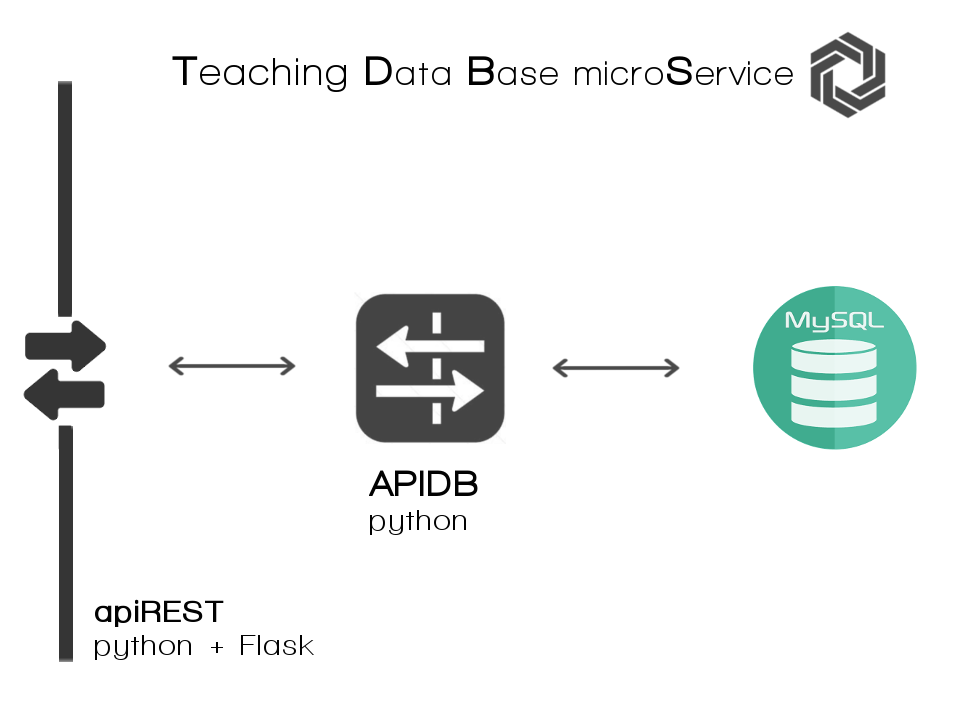
\includegraphics[scale=0.35]{img/graphics/tdbms.png}
\end{center}

\subsection{Api definition}
\begin{lstlisting}[language=python,frame=none]

  #%RAML 0.8
  title: Teaching Data Base API
  version: 1.0
  baseUri: ---

  /test:
    description:
    get:
      description:
      responses:
        200:
          description: Ok. Successful requests.

  /test_mysql:
    description:
    get:
      description:
      responses:
        200:
          description: Ok. Successful requests.

  /entities/{kind}:
    description:
    get:
      description:
      responses:
    post:
      description: INSERT a entity in the database, with a special input format:
      responses:

  /entities/{kind}/{entity_id}:
    description:
    get:
      description:
      responses:
        200:
          description:
    put:
      description:
      responses:
        201:
    delete:
      description:
      respones:
        204


  /entities/{kind}/{entity_id}/{nested_kind}/{onk_entity_id}:
  description:

    delete:
      description:
      respones:
        204

  /entities/{kind}/{entity_id}/{related_kind}:
  description:
  get:
    description:
    responses:
      200:
        description:

  /entities/{kind}/{entity_id}/{relared_kind}/{rk_entity_id}/{subrelated_kind}:
  description:
  get:
    description:
    response:
      200:
        description:

  /entities/{kind}/{entity_id}/report:
  description:
  get:
    description:
    response:
      200:
        description:



\end{lstlisting}




\subsubsection{Database logical design}

Based on user histories and the domain of the problem the designe
done based of this entity relation diagram:

The design follow some details that the domain presents, that is related
(at least the more significantly) below:

\begin{center}
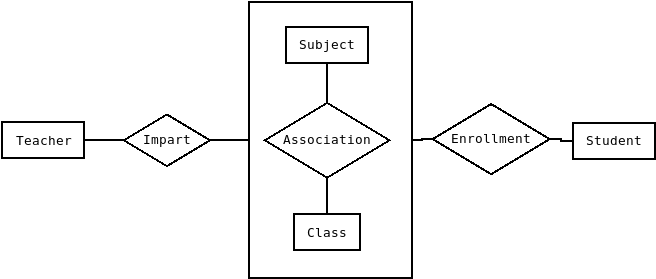
\includegraphics[scale=0.4]{img/diagrams/dbms-ER.png}
\end{center}



\subsubsection{Way to access to raw data}

While at firs of develop the mainly strategie to follow was write
all by cero, finally the point of view has been changed to follow
the use of standard tools and avoid reinvent the wheel.
\intro
So, if in the first stages of the project the acces to raw data through
the engine was hand made, using an own simple library that worked
like as simple ORM, the evolution of it and especially the problems
found and the unmaintainability of code have made that now the approach
turned to use a good tool as ORM like \href{http://www.google.es}{SQLAlchemy}.
\intro
The changes in the specifications of the api while the develop and
the maintaince of the performance of the queries when is writed hand
made in raw SQL isn't a good idea. Before the develop of this mService
it easy to understand that only in few projects is justified the use
of raw sql sencences and drivers whiout ORM (by easy that it was).


\section{Students Control microService}

\subsection{Domain and design}

\begin{center}
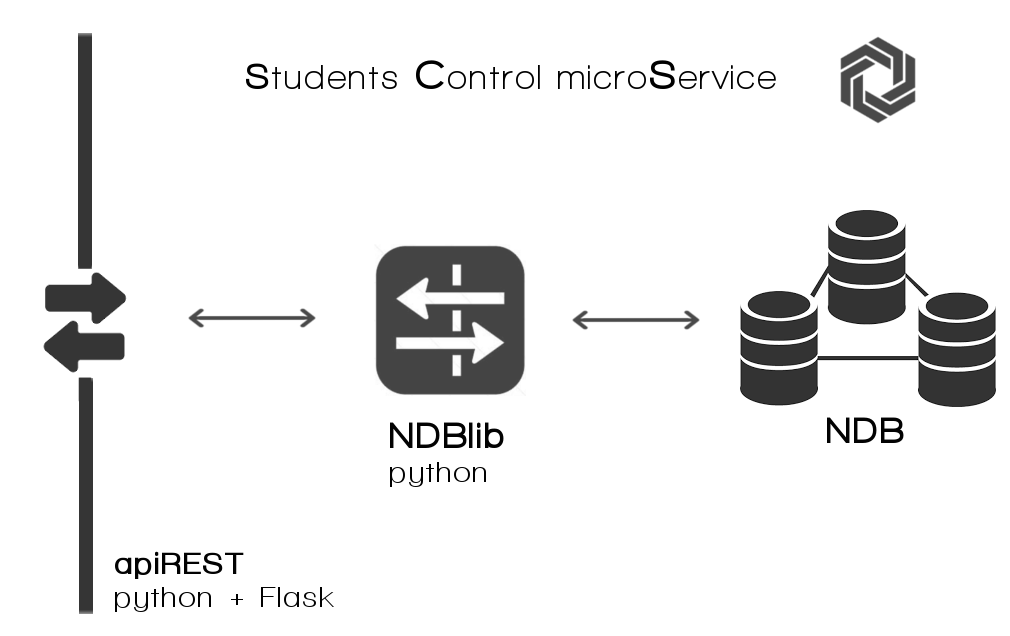
\includegraphics[scale=0.4]{img/graphics/scms.png}
\end{center}

\subsection{Api definition}

skjsñdf
asflkafkdafldañfdsfl


\subsubsection{Attendance Controls Subsection}

This is a simple collection behaviour resource.

This is a RAML0.8 definition file:

\begin{lstlisting}[language=python,frame=none]

  #%RAML 0.8
  title: Attendance Controls API
  version: 1.0
  baseUri: ---
  /ac:
    description: The resource to work with attendance controls database saved-
    get:
      description: Get a list of all attendance controls
      responses:
        200:
          description: Ok. Successful requests. An item will be returned.

    post:
      description:
      responses:
        201:
          description: Created without response. The item was added to database will not
                       returned body.
        422:
          description: Unprocessable Entity. Probably because of the payload
                       sendes has not correct format.

    /{ac_id}:
      uriParameters:
       ac_id:
         displayName: Attendance control ID
         type: integer
      get:
        description: Return an item of the attendance controls collection.
        responses:
          200:
            description: Ok. Successful requests. An item will be returned.
          404:
            description: Not found. The item required does not exists.
      put:
        description: Save a new attendance control in the database.
        responses:
          204: No content. The server has fulfilled the request but does not need to return an entity-body.
          404:
            description: Not found. The item required does not exists.

      delete:
        description:
        responses:
          204: No content. The server has fulfilled the request but does not need to return an entity-body.
          404:
            description: Not found. The item required does not exists.

    /schema:
      uriParameters:
       ac_id:
         displayName: Attendance control ID
         type: integer
      get:
        description:
        responses:
          200:
            description: Ok. Successful requests. An item will be returned.
          404:
            description: Not found. The item required does not exists.

\end{lstlisting}

\subsubsection{Disciplinary Notes Subsection}

This is a simple collection behaviour resource.

This is a RAML0.8 definition file:

\begin{lstlisting}[language=python,frame=none]

  #%RAML 0.8
  title: Attendance Controls API
  version: 1.0
  baseUri: ---
  /ac:
    description: The resource to work with attendance controls database saved-
    get:
      description: Get a list of all attendance controls
      responses:
        200:
          description: Ok. Successful requests. An item will be returned.

    post:
      description:
      responses:
        201:
          description: Created without response. The item was added to database will not
                       returned body.
        422:
          description: Unprocessable Entity. Probably because of the payload
                       sendes has not correct format.

    /{ac_id}:
      uriParameters:
       ac_id:
         displayName: Attendance control ID
         type: integer
      get:
        description: Return an item of the attendance controls collection.
        responses:
          200:
            description: Ok. Successful requests. An item will be returned.
          404:
            description: Not found. The item required does not exists.
      put:
        description: Save a new attendance control in the database.
        responses:
          204: No content. The server has fulfilled the request but does not need to return an entity-body.
          404:
            description: Not found. The item required does not exists.

      delete:
        description:
        responses:
          204: No content. The server has fulfilled the request but does not need to return an entity-body.
          404:
            description: Not found. The item required does not exists.

    /schema:
      uriParameters:
       ac_id:
         displayName: Attendance control ID
         type: integer
      get:
        description:
        responses:
          200:
            description: Ok. Successful requests. An item will be returned.
          404:
            description: Not found. The item required does not exists.

\end{lstlisting}

\subsubsection{Maks Subsection}

This is a simple collection behaviour resource.

This is a RAML0.8 definition file:

\begin{lstlisting}[language=python,frame=none]

  #%RAML 0.8
  title: Attendance Controls API
  version: 1.0
  baseUri: ---
  /ac:
    description: The resource to work with attendance controls database saved-
    get:
      description: Get a list of all attendance controls
      responses:
        200:
          description: Ok. Successful requests. An item will be returned.

    post:
      description:
      responses:
        201:
          description: Created without response. The item was added to database will not
                       returned body.
        422:
          description: Unprocessable Entity. Probably because of the payload
                       sendes has not correct format.

    /{ac_id}:
      uriParameters:
       ac_id:
         displayName: Attendance control ID
         type: integer
      get:
        description: Return an item of the attendance controls collection.
        responses:
          200:
            description: Ok. Successful requests. An item will be returned.
          404:
            description: Not found. The item required does not exists.
      put:
        description: Save a new attendance control in the database.
        responses:
          204: No content. The server has fulfilled the request but does not need to return an entity-body.
          404:
            description: Not found. The item required does not exists.

      delete:
        description:
        responses:
          204: No content. The server has fulfilled the request but does not need to return an entity-body.
          404:
            description: Not found. The item required does not exists.

    /schema:
      uriParameters:
       ac_id:
         displayName: Attendance control ID
         type: integer
      get:
        description:
        responses:
          200:
            description: Ok. Successful requests. An item will be returned.
          404:
            description: Not found. The item required does not exists.

\end{lstlisting}



\section{Analysis microService}

\subsection{Domain and design}
\begin{center}
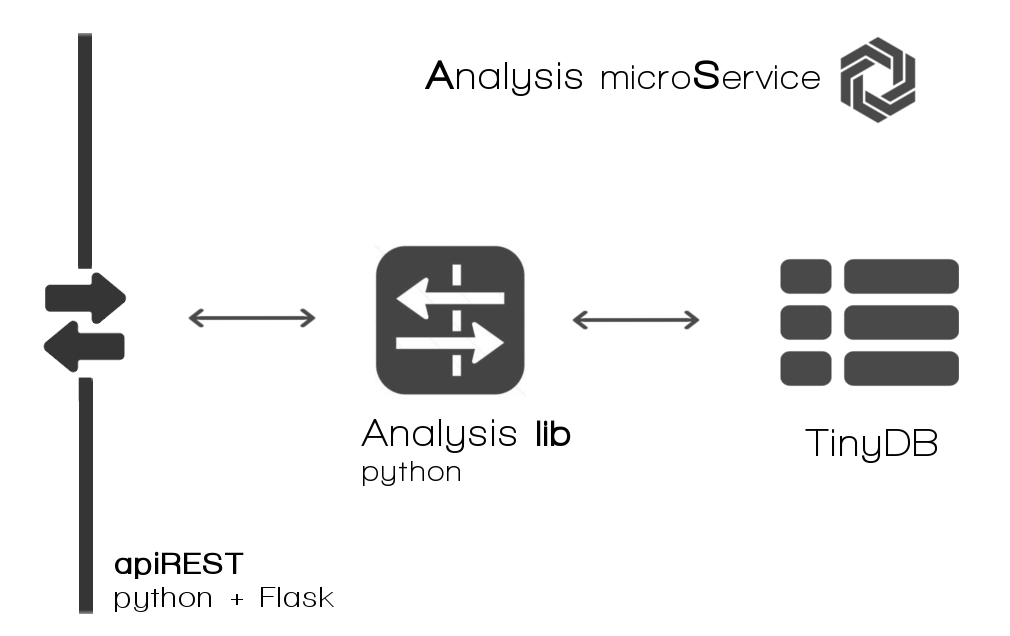
\includegraphics[scale=0.4]{img/graphics/ams.png}
\end{center}


\section{User Interface microService}

\subsection{Domain and design}
\begin{center}
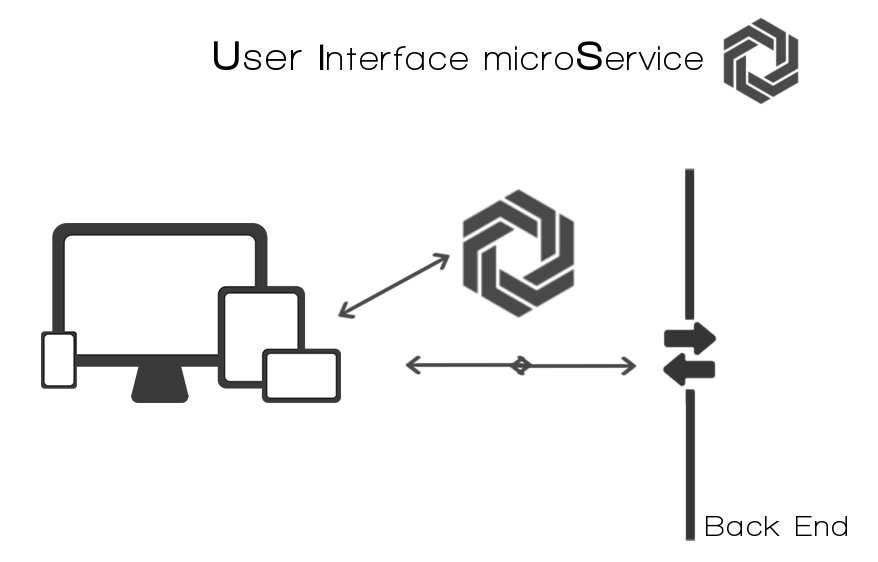
\includegraphics[scale=0.4]{img/graphics/ui.png}
\end{center}


\section{Auxiliar tools}


\subsection{Provisioner}
A provisioner is simply a tool used to provide a system to insert test data, to
avoid to do this hand-made, in our services.

\begin{center}
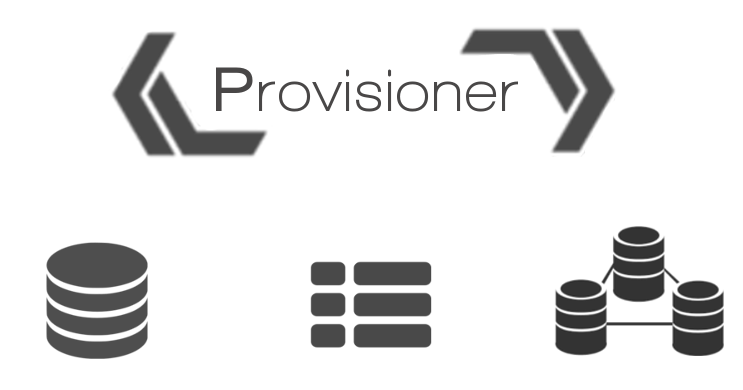
\includegraphics[scale=0.4]{img/graphics/provisioner.png}
\end{center}

\noindent Normally this work without knowledge
of the internal parts of the backend, only working with their API gateway (or
API if we want only fill the database of service), understanding it as a black box.
this is only an approach, we can design our provisioner to fill data directly
in the databases, which will require established a connection with them without
the interaction of the services or their connection libraries. This is faster but
on some occasions, we do not want to do this, because another of their goal is to
check at the same time the correctly of all parts of APIs involved in the data insertion.
\intro
So, the execution this kind of program required that the system has fully launched.
This will be the most used tool when we want to try some feature that required a
lot of data in the system.
\intro
How does it work? Easy, only need simple parameters as entry and based on some rules it will do all
calls to the API gateway to insert all data required, besides to save all operations
in a register or log file because is necessary to check this in a debug operation.
